
\chapter{Návrh grafického programovacieho jazyka}
\label{kap:navrh-gpj}

V kapitole opisujeme priebeh vzniku grafického programovacieho jazyka použitého v našej aplikácii. Rôzne verzie (kapitola \ref{sec:system-verzii}) vyžadujú sprístupnenie rôznych komponentov. Hlavným predmetom tvorby GPJ pomocou knižnice Blockly je definícia blokov a im prislúchajúcich generátorov (kapitola \ref{kap:GrafickyProgramovaciJayzk}).


%%%%%
% %%% 	Verzia Otto 2020 Robotická liga
%%%%%
\section{Verzia Otto 2020 Robotická liga}
V tejto verzii je možné tvoriť choreografie pre robota Otto ako postupnosť trojíc celých čísel (kapitola \ref{sub:otto} a \ref{sub:verzia-otto-2020-rl}). Formát a význam jednotlivých čísel je uvedený na web stránke Denného tábora digitálnych technológií prezentujúcej robota Otto \cite{ottoChoreographies}. Základom sú trojice pre ovládanie motorov, k dispozícii sú ale i ďalšie, umožňujúce ovládanie prehrávania melódie či zvukových efektov (tabuľka \ref{tab:otto-choreograpies-tab}). Celá choreografia, sériovou linkou prenášaná do mikropočítača, má formát \uv{$@\;x_1\;y_1\;z_1\;x_2\;y_2\;z_2\;...\;x_n\;y_n\;z_n\;0\;0\;0 $}, kde vždy trojica (príkaz) pozostáva z hodnôt ($x_i, y_i, z_i$).

\begin{table}\footnotesize
\centering
\newcolumntype{P}[1]{>{\centering\arraybackslash}p{#1}}
\begin{tabular}{ |P{1cm}P{0.6cm}P{1cm}|p{11.2cm}| }
	\hline
	\multicolumn{3}{|c|}{\textbf{formát príkazu}}&\textbf{význam} \\
	\hline
	$X$ & $Y$   & $Z$ & počkaj $X$ ms, pohni motorom $Y$ do polohy $Z$; $Y\in [1;6]; Z\in [0,180]$  \\
	1 & 8   & $X$ & nastav celkový čas prehrávania choreografie na $X$ sekúnd \\
	1 & 9   & $X$ & pokračuj príkazom na riadku $X$ \\
	1 & 10 & $X$ & nastav spomalenie pohybu, 0= bez spomalenia \\
	1 & 11 & $X$ & začni hrať melódiu číslo $X$, 0 = vypnúť zvuk \\
	1 & 12 & $X$ & zahraj zvukový efekt číslo $X$ \\
	1 & 13 & 0 & zastav prehrávanie melódie \\
	1 & 14 & $X$ & začni hrať pesničku číslo $X$ \\
	1 & 15 & 0 & vypni / zapni reproduktor \\
	\hline
 \end{tabular}
\caption{\label{tab:otto-choreograpies-tab}Prípustné hodnoty v zápise choreografie robota Otto pomocou trojíc čísel}
\end{table}\normalsize

Na základe tabuľky \ref{tab:otto-choreograpies-tab} vytvárame v GPJ bloky pre jednotlivé funkcie (trojice). Cieľom je zachovať rozsah funkcionalít, no ponúknuť atraktívnejší a pohodlnejší prístup k tvorbe choreografie tohoto formátu. Jednotlivé bloky sú interpretované jednoducho ako prislúchajúca trojica celých čísel.

Príklad choreografie vytvorenej pomocou vzniknutých blokov možno vidieť na obrázku \ref{obr:otto-rl-blockly-general-example}. Bloky vyžadujúce zadanie parametra majú v tele dostupné pole, kde je možné príslušnú hodnotu určiť. Na obrázku \ref{obr:otto-rl-blockly-general-example} ide napríklad o bloky pre nastavenie spomalenia alebo blok pre spustenie prehrávania melódie. V prípade bloku pre riadenie pohybu motora zavádzame možnosť výberu konkrétneho motora z ponuky, namiesto zadania jeho čísla. Zavádzame tiež blok \uv{Program}, do ktorého tela sú vkladané ostatné bloky --- prvky choreografie. Blok \uv{Program} je v tejto verzii statickým prvkom pracovnej plochy editora GPJ, používateľ ho nemôže odstrániť ani duplikovať. Slúži na ohraničenie blokov, ktoré tvoria choreografiu. Bloky umiestnené v editore mimo telo tohto bloku nie sú brané do úvahy pri generovaní kódu. Výsledný program po preložení blokov môžete vidieť v ukážke \ref{OttoRlGeneralExampleCode}.

\begin{figure}
\centerline{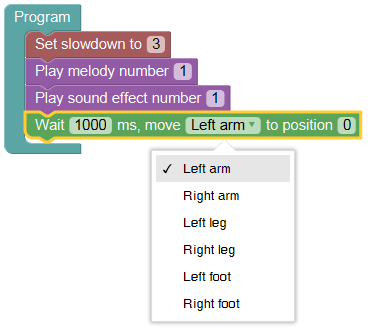
\includegraphics[width=0.6\textwidth]{images/otto-rl-blockly-general}}
\caption[Ukážka kódu v GPJ pre verziu Otto RL 2020]{Ukážka kódu v GPJ pre verziu Otto RL 2020}
\label{obr:otto-rl-blockly-general-example}
\end{figure}

\lstset{language=C,caption={Kód generovaný z blokov na obrázku \ref{obr:otto-rl-blockly-general-example}},label=OttoRlGeneralExampleCode}
\begin{lstlisting}[frame=single]
@1 10 3
1 11 1
1 12 1
1000 5 0
0 0 0
\end{lstlisting}


%%%%%
% %%% 	Verzia Otto 2021 Procedural
%%%%%
\section{Verzia Otto 2021 Procedural}
V tejto verzii sprístupňujeme v GPJ prvky pre tvorbu riadiaceho programu v jazyku Arduino (C++). Použité bloky sú členené do kategórií. Každá kategória zodpovedá \uv{tematickému} celku, prípadne logickému modulu verzie. Podľa zavedených kategórií sú bloky zobrazené v ponuke v používateľskom rozhraní. Nižšie uvádzame ich zoznam.

\begin{itemize}[topsep=8pt,itemsep=0.1pt,partopsep=4pt, parsep=4pt]
\item Matematická logika (podmienka if, logické operácie, pravdivostné hodnoty)
\item Cykly (cyklus for, while a blok pre príkazy \textit{break} a \textit{continue})
\item Matematika (číselné konštanty, aritmetické operácie, náhodné čísla)
\item Premenné (tvorba premenných rôznych typov)
\item Funkcie (tvorba procedúr a funkcií)
\item Zvuk (ovládanie zvukových efektov a mp3 prehrávača)
\item Pohyb (ovládanie servomotorov)
\item Senzory (prístup k funkciám dotykových tlačidiel a ultrazvukovému senzoru)
\item Sériová komunikácia prostredníctvom USB
\item Sériová komunikácia prostredníctvom Bluetooth
\item Práca s časom
\item Kontrola batérií
\end{itemize}

Knižnica Blockly poskytuje základné, všeobecné bloky \uv{od výroby}. K dispozícii sú bloky pre \textit{vetvenie programu podmienkou if}, bloky pre \textit{cykly}, bloky pre \textit{logické a číselné konštanty} a manipuláciu s nimi (základná aritmetika a logické operácie), bloky pre \textit{manipuláciu s textom}, \textit{tvorbu zoznamov}, \textit{reprezentáciu a miešanie farieb}, \textit{tvorbu premenných} a \textit{definíciu procedúr a funkcií}. Súčasťou sú generátory pre jazyky JavaScript, Python, Dart, Lua a PHP, z ktorých možno vychádzať. Niektoré z týchto blokov použijeme i v našej aplikácii, najmä definíciu ich vizuálnej podoby. Syntax jazyka C však vyžaduje redefiníciu generátorov viacerých prebraných blokov. K prebraným častiam patria bloky pre logické operácie, cykly, definície procedúr a funkcií, matematické operácie a premenné. Dôležitými pre našu aplikáciu sú však najmä novovzniknuté bloky, umožňujúce obsluhu špecifických funkcií robota. V knižnici dotvárame bloky umožňujúce pohyb, čítanie hodnôt meraných senzormi, sériovú komunikáciu či komunikáciu rozhraním Bluetooth. 

Komplexitou funkcie poskytovanej blokom je možné nastaviť úroveň abstrakcie. Jednoduchým príkladom je blok \uv{čakanie na stlačenie tlačidla} (obrázok \ref{obr:wait-till-couch}). Možno ho ľahko vyskladať z blokov \textit{cyklu while}, \textit{negácie} a bloku pre \textit{načítanie stavu tlačidla} (na obrázku vľavo), no najmä pre nižšie vekové kategórie je vhodnejšia alternatíva vyššej abstraktnej úrovne (na obrázku vpravo). Iným príkladom je blok pre načítanie gesta pomocou ultrazvukového senzora, ktorý reprezentuje v pozadí pomerne zložitú implementáciu časti riadiaceho programu, zabezpečujúcu komunikáciu s hardvérom a elimináciu chyby opakovaným meraním. V rámci jednotlivých kategórií je preto našou snahou poskytnúť bloky rôzneho charakteru, s rôznou úrovňou abstrakcie.

\begin{figure}
\centerline{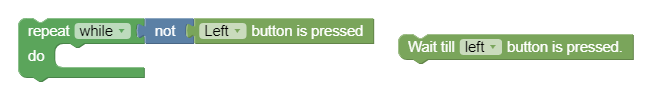
\includegraphics[width=1\textwidth]{images/wait-till-couch}}
\caption[Abstrakcia bloku \uv{čakaj na stlačenie tlačidla}]{Abstrakcia bloku \uv{čakaj na stlačenie tlačidla}}
\label{obr:wait-till-couch}
\end{figure}

I v tejto verzii zavádzame v editore GPJ fixný, statický blok \uv{Program}, ktorý reprezentuje časť \textit{loop} riadiaceho programu a všetok kód je tvorený pridávaním blokov do jeho tela. Bloky bez pripojenia (priameho a zároveň nepriameho) k tomuto bloku nie sú pri vyhodnocovaní (generovaní kódu) brané do úvahy. Výnimku majú len bloky umiestnené v tele blokov definujúcich funkcie a procedúry. Príklad možno vidieť na obrázku \ref{obr:disabled-orphan-block}. Je tu zobrazený obsah pracovnej plochy editora GPJ. Blok vľavo bude pri generovaní C++ kódu vyhodnotený, ide o hlavný blok \uv{Program}, ktorého obsah tvorí časť \textit{loop} riadiaceho programu. Blok v strede, definujúci procedúru \uv{do something}, bude tiež vyhodnotený a pripojený v generovanom kóde za časť \textit{loop}, aby bolo možné procedúru z časti \textit{loop} volať. Blok pre cyklus (na obrázku vpravo) bude pri vyhodnocovaní ignorovaný, nakoľko nie je priamym ani nepriamym potomkom bloku \uv{Program} ani bloku definujúceho procedúru alebo funkciu. Tento stav je používateľovi signalizovaný vizuálne zblednutím bloku.

\begin{figure}
\centerline{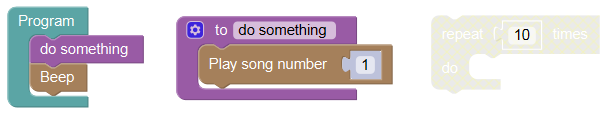
\includegraphics[width=0.95\textwidth]{images/disabled-orphan-block}}
\caption[Blok umiestnený mimo hlavného programu a definície procedúry]{Blok umiestnený mimo hlavného programu a definície procedúry}
\label{obr:disabled-orphan-block}
\end{figure}

% zakladne bloky, logika, cykly, aritmetika
\subsection{Základné bloky, logika, cykly, aritmetika}
Definície blokov kategórií \textit{matematická logika}, \textit{cykly} a \textit{matematika} preberáme od autorov knižnice Blockly. Pri definícii generátora vychádzame z existujúceho, produkujúceho kód v jazyku JavaScript. V aplikácii sú prístupné bloky pre podmienku if, konštanty pravdivostných hodnôt a ich porovnanie, blok pre negáciu, číselné konštanty, unárne mínus, aritmetické operácie a blok pre prístup ku generátoru náhodných čísel. Vyššiu abstrakciu pre logické operácie poskytuje napríklad blok \uv{test vlastnosti čísla} (obrázok \ref{obr:block-number-property}), ktorého návratovou hodnotou je pravdivostná hodnota a používateľovi umožňuje testovať paritu, pozitivitu alebo deliteľnosť čísel na základe slovnej definície tejto vlastnosti. Generátor tento blok do jazyka C++ následne preloží ako príslušnú logickú operáciu, napríklad blok \uv{$x$ je pozitívne} je prekladaný ako \uv{$x\ge0$}, blok \uv{$y$ je párne} bude interpretovaný ako \uv{$y\; \% \;2\; ==\; 0)$} 

V kategórii cyklov (obrázok \ref{obr:loop-blocks}) sú k dispozícii bloky pre štandardný cyklus for, while, blok pre príkaz \textit{break} a \textit{continue}. Vyššiu abstrakciu umožňuje špeciálny cyklus, pre ktorý používateľ definuje len počet iterácií (na obrázku vpravo dole). Pri generovaní kódu je potom na jeho mieste vytvorená definícia štandardného cyklu \textit{for} s lokálnou premennou, ktorou je iterované v postupných inkrementoch od 0 po užívateľom zadané číslo - 1. Vnútri bloku tohto cyklu môžete vidieť spomínaný blok pre príkazy \textit{break} a \textit{continue}, charakter tohto bloku možno zvoliť výberom z možností.

\begin{figure}
\centerline{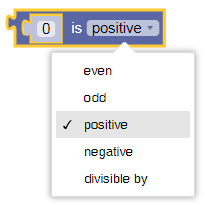
\includegraphics[]{images/block-number-property}}
\caption[Abstrakcia bloku testujúceho vlastnosť čísla]{Abstrakcia bloku testujúceho vlastnosť čísla}
\label{obr:block-number-property}
\end{figure}

\begin{figure}
\centerline{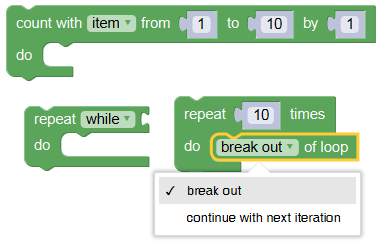
\includegraphics[]{images/loop-blocks}}
\caption[Bloky v kategórii \textit{cykly}]{Bloky v kategórii \textit{cykly}}
\label{obr:loop-blocks}
\end{figure}

% premenne
\subsection{Premenné}
Dôležitým komponentom jazyka sú premenné. Blockly je potrebné prispôsobiť pre použitie typových premenných jazyka C, pričom autori podobných aplikácií pristupujú k riešeniu premenných rôzne. V online webovej verzií editora MakeCode (riadenie robota Lego Mindstorms) sú k dispozícii len číselné premenné, textové reťazce a binárne hodnoty môžu byť len konštantou \cite{makeCodeWebEditor}. Na druhej strane, v produkte Otto Blockly je možné vytvoriť premennú typu znak, reťazec, celé číslo, desatinné číslo i binárna hodnota. K dispozícií sú bloky pre inicializáciu, priradenie, i získanie hodnoty premennej. Typy nie sú však vizuálne výraznejšie odlíšené. V editore kódu možno deklarovať premennú binárneho typu a následne iným blokom túto premennú inkrementovať, na čo validátor bloku oznámi chybu. Otázne však je, či je vhodné povoliť vytvorenie neprípustného spojenia.

V našej aplikácii vynucujeme určenie typu premennej pri jej vytváraní, bez možnosti dodatočnej zmeny. Povolené typy sú binárna hodnota (bool), celé číslo (int16\_t) a textový reťazec (String). Bloky pre priradenie do premennej a čítanie premennej majú pre jednoznačnosť v rámci typu rovnakú farbu (obrázok \ref{obr:variables-blocks}). Správnosť typu je vynucovaná pri každom pokuse o spojenie blokov. V rámci blokov pre priradenie do premennej (horný rad blokov na obrázku \ref{obr:variables-blocks}) a blokov pre čítanie hodnoty z premennej (dolný rad blokov na obrázku \ref{obr:variables-blocks}) je k dispozícii ponuka pre výber inej premennej rovnakého typu.

Premenné sú používateľom tvorené kliknutím na tlačidlo v ponuke prvkov GPJ v kategórii /textit{premenné}. Pre vytvorenie konkrétneho typu je k dispozícii separátne tlačidlo. V tejto sekcii sú tiež k dispozícii bloky pre čítanie a zápis do každej vytvorenej premennej. Iným spôsobom pre vytvorenie premennej je jej deklarovanie v zozname parametrov procedúry alebo funkcie, či použitie cyklu \textit{for}, kde je automaticky zavedená iteračná premenná typu \textit{číslo}.

\vspace{3cm}

\begin{figure}[bh!]
\centerline{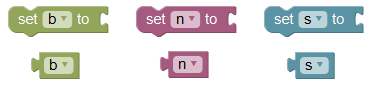
\includegraphics[]{images/variables-blocks}}
\caption[Bloky v kategórii \textit{premenné}]{Bloky v kategórii \textit{premenné}}
\label{obr:variables-blocks}
\end{figure}

\newpage

% procedury a funkcie
\subsection{Procedúry a funkcie}
Bloky pre vytváranie procedúr a funkcií boli modifikované pre podporu typových premenných. V definícii funkcie je nutné deklarovať typ parametrov a pri volaní je následne vynucovaný. Pre tento účel bola rozšírená ponuka dialógového okna pre úpravu počtu parametrov funkcie (obrázok \ref{obr:function-definition}).

Komplikáciou pri práci s procedúrami a funkciami je určenie rozsahu platnosti premenných, ich argumentov. V Blockly je pre vytváranie blokov umožňujúcich manipuláciu s premennými štandardne určená jedna z kategórií menu ponuky prvkov GPJ. Sú v nej zobrazené všetky vytvorené premenné, lokálne i globálne, všetky, čo boli v editore deklarované. Môže tak ľahko dôjsť k zmätočnej situácii, keď deklarujeme rovnomennú premennú iného typu v rámci dvoch procedúr a v menu sú naraz dostupné obe. Riešením je vynucovanie typu pre raz definovaný názov premennej. Takto možno všetky používateľom vytvorené premenné vyhlásiť za globálne a predísť nežiadaným situáciám.

Blok pre definíciu funkcie bol modifikovaný doplnením pola pre explicitnú špecifikáciu návratového typu (pole pre výber možností, na obrázku \ref{obr:function-definition} je zobrazené v pravej dolnej časti bloku, zobrazuje hodnotu \uv{Boolean}).

\vspace{3cm}

\begin{figure}[bh!]
\centerline{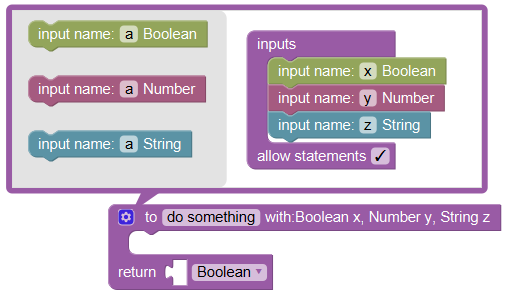
\includegraphics[]{images/function-definition}}
\caption[Definícia argumentov funkcie]{Definícia argumentov funkcie}
\label{obr:function-definition}
\end{figure}

\newpage

% zvuk
\subsection{Zvukové efekty a mp3 prehrávač}
Bloky v tejto kategórii umožňujú ovládať výstupné zariadenia robota, sirénu a mp3 prehrávač. Poskytujú vysokú abstrakciu nad procesmi v mikropočítači, ktoré zabezpečujú požadovaný výsledný efekt. Pri práci s melódiami (sirénou) je napríklad v mikropočítači implementovaná práca s časovačom, ktorý na základe preddefinovanej postupnosti hodnôt tvorí signály reprezentujúce tóny, následne odosielané do súčiastky tvoriacej zvuk. Implementáciu tejto časti preberáme z pôvodnej verzie riadiaceho programu robota Otto, vyvinutého pre účely denných táborov (kapitola \ref{sub:otto}). Vznikli tak bloky pre vydanie konkrétneho tónu ale i komplexnejšie, pre zahranie celej preddefinovanej melódie a pre prehranie niekoľkých predpripravených zvukových efektov (obrázok \ref{obr:sound-blocks}). Bloky sú parametrizované, číselné hodnoty možno buď to zadať manuálne (konštantou) alebo použitím bloku s výstupom typu \textit{číslo}, napríklad premennej.

Pre ovládanie mp3 prehrávača vznikli bloky pre spustenie konkrétnej skladby, pozastavenie a obnovenie prehrávania, úpravu hlasitosti a blok pre načítanie aktuálne zvolenej hlasitosti (obrázok \ref{obr:mp3-blocks}). I v tomto prípade zabezpečujú bloky vysokú abstrakciu nad procesom v pozadí. Mp3 prehrávač je riadený odosielaním riadiacich inštrukcií v preddefinovanom formáte.

Pre prehľadnosť kódu tvoreného prekladom použitých blokov je generátorom GPJ vytvorené len volanie funkcie definovanej v pomocných súboroch daného logického modulu verzie (kapitola \ref{sec:system-verzii}). Pre ilustráciu uvažujme blok \uv{Prehrať pesničku číslo $x$}. Pre tento úkon je nutné odoslať z mikropočítača do mp3 prehrávača sekvenciu riadiacich inštrukcií \cite{DFPlayerMini}. Blok je preložený ako \uv{jednoduché} volanie funkcie \uv{mp3\_play($x$)}, ktorej definícia je umiestnená vo \textit{footer} súbore logického modulu \textit{zvuk}. Implementáciu pomocnej funkcie (a s ňou súvisiacich funkcií) pre tento blok uvádzame v ukážke \ref{playSongSupportFunctions}.

\vspace{2cm}

\begin{figure}[bh!]
\centerline{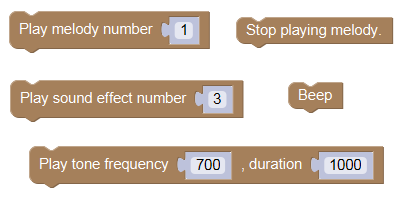
\includegraphics[]{images/sound-blocks}}
\caption[Bloky pre ovládanie zvukových efektov]{Bloky pre ovládanie zvukových efektov}
\label{obr:sound-blocks}
\end{figure}

\newpage

\lstset{language=C,caption={Pomocné funkcie pre blok \uv{Prehrať pesničku číslo $x$}},label=playSongSupportFunctions,basicstyle=\footnotesize}
\begin{lstlisting}[frame=single]
void mp3_play(uint8_t song_number) {
  mp3_send_packet(0x03, song_number);
}

void mp3_send_packet(uint8_t cmd, uint16_t param) {
  mp3_send_byte(MP3_OUTPUT_PIN, 0x7E);
  mp3_send_byte(MP3_OUTPUT_PIN, 0xFF);
  mp3_send_byte(MP3_OUTPUT_PIN, 0x06);
  mp3_send_byte(MP3_OUTPUT_PIN, cmd);
  mp3_send_byte(MP3_OUTPUT_PIN, 0x00);
  mp3_send_byte(MP3_OUTPUT_PIN, (uint8_t)(param >> 8));
  mp3_send_byte(MP3_OUTPUT_PIN, (uint8_t)(param & 0xFF));
  uint16_t chksm = 0xFF + 0x06 + cmd + (param >> 8) + (param & 0xFF);
  chksm = -chksm;
  mp3_send_byte(MP3_OUTPUT_PIN, (uint8_t)(chksm >> 8));
  mp3_send_byte(MP3_OUTPUT_PIN, (uint8_t)(chksm & 0xFF));
  mp3_send_byte(MP3_OUTPUT_PIN, 0xEF);
}

void mp3_send_byte(uint8_t pin, uint8_t val) {
  pinMode(MP3_OUTPUT_PIN, OUTPUT);
  float start_transmission = micros();
  float one_bit = 1000000 / 9600.0;
  float next_change = start_transmission + one_bit;
  digitalWrite(pin, LOW);
  while (micros() < next_change);
  
  for (int i = 2; i < 10; i++) {
    if (val & 1) digitalWrite(pin, HIGH);
    else digitalWrite(pin, LOW);
    next_change = start_transmission + one_bit * i;
    val >>= 1;
    while (micros() < next_change);
  }

  digitalWrite(pin, HIGH);
  next_change = micros() + 2 * one_bit;
  while (micros() < next_change);
  pinMode(MP3_OUTPUT_PIN, INPUT);
}
\end{lstlisting}

\begin{figure}
\centerline{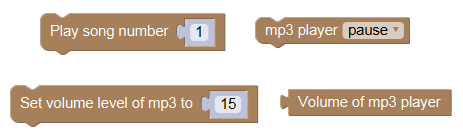
\includegraphics[]{images/mp3-blocks}}
\caption[Bloky pre ovládanie mp3 prehrávača]{Bloky pre ovládanie mp3 prehrávača}
\label{obr:mp3-blocks}
\end{figure}

\newpage

%pohyb
\subsection{Pohyb}
Pre ovládanie servomotorov robota bolo v GPJ vytvorených niekoľko blokov (obrázok \ref{obr:move-blocks}). Základným je blok pre natočenie konkrétneho motora do konkrétnej polohy (na obrázku \ref{obr:move-blocks} hore), z ktorého by s použitím ostatných prvkov GPJ bolo možné vyskladať všetky ďalšie, komplexnejšie.

Pre vyššiu úroveň abstrakcie slúžia bloky ako \uv{reset pozícií motorov}, ktorý spôsobí postupné natočenie všetkých motorov do polohy 90 stupňov. Robota tak možno ľahko priviesť do iniciálnej pozície v stoji s upaženými rukami. Bloky \uv{stoj na špičkách}, \uv{stoj na pätách} a \uv{zamávaj rukou} sú jednoduchými gestami, spájajúcimi postupný pohyb niekoľkých motorov. Bloky \uv{choď vpred} a \uv{otoč sa vľavo} (v poli dostupnom na blokoch možno tiež zvoliť opačný smer, vzad a vpravo) predstavujú komplexný pohyb, ich implementácia je inšpirovaná pôvodným riadiacim programom pre robota Otto a v podporných súboroch logického modulu \textit{pohyb} sú implementované ako prehrávanie krátkej choreografie. Tieto komplexné pohyby sú navrhnuté tak, aby predstavovali jeden ucelený pohyb s pokiaľ možno rovnakou východiskovou a cieľovou polohou všetkých zapojených motorov. Napríklad blok \uv{choď vpred} by sa dal inak pomenovať ako \uv{krok vpred}. Pre chôdzu robota je tak nevyhnutné tento blok umiestniť do cyklu. Rovnaký princíp platí pre blok otáčania. Nie je tu definovateľná miera natočenia, nakoľko nevieme s istotou povedať, že ju dosiahneme určitou sériou elementárnych pohybov jednotlivými motormi.

\begin{figure}[bh!]
\centerline{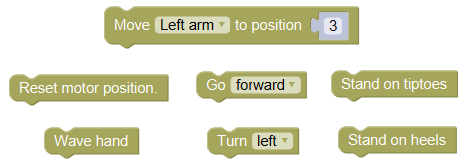
\includegraphics[]{images/move-blocks}}
\caption[Bloky pre ovládanie servomotorov]{Bloky pre ovládanie servomotorov}
\label{obr:move-blocks}
\end{figure}

\newpage

%senzory
\subsection{Senzory}
V tejto kategórii je tiež uplatnená vysoká miera abstrakcie. Pre obsluhu dotykových senzorov o čosi menšia, napríklad blok zisťujúci, či je tlačidlo práve stlačené, prekladá generátor priamo na funkciu \uv{digitalRead(TOUCH1)}, kde \textit{digitalRead} je funkcia prístupná v jazyku Arduino, návratovou hodnotou je pravdivostná hodnota, určujúca, či je na danom pine detegované pozitívne napätie. Parameter \textit{TOUCH1} určuje číslo pinu, v ktorom je dane tlačidlo zapojené, táto konštanta je definovaná v pomocnom \textit{header} súbore logického modulu \textit{senzory}. Bloky vyššej abstrakcie tu reprezentujú \uv{čakanie na stlačenie tlačidla}. V tomto prípade je vygenerovaný krátky blok kódu, cyklicky kontrolujúci hodnotu prijímanú na pine prislúchajúcom tlačidlu, kým nie je detegované stlačenie. Vysokú abstrakciu dovoľuje blok pre \uv{načítanie gesta}. V tomto prípade je vykonaná funkcia detegujúca počet stlačení tlačidla. Jej implementáciu môžete vidieť v ukážke \ref{touchGestureRecordFunction}. Pre elimináciu chyby je gesto (jedno zo stlačení) registrované až po niekoľkonásobnej detekcii stlačenia v určitom časovom intervale. Implementácie tiež umožňuje zadanie gesta dlhým stlačením. Po určitom intervale neprestajného \uv{stlačenia} je zaznamenané ďalšie \uv{stlačenie}. Zadávanie gesta je ukončené po neregistrovaní stlačenia po definovaný čas. Súčasťou blokov pre interakciu s dotykovými senzormi je možnosť voľby senzora (robot Otto má dva).

Pre ultrazvukový senzor boli bloky navrhnuté analogicky. Aktuálne meranú vzdialenosť možno načítať blokom \uv{Ultrazvuk vzdialenosť} (návratová hodnota je číslo --- vzdialenosť v centimetroch), namiesto stlačenia je tu možnosť vyčkávať na detekciu vzdialenosti menšej alebo väčšej ako používateľom zadaná hodnota. Gesto je vyjadrené počtom nameraní vzdialenosti do 50 centimetrov (analógia stlačenia tlačidla).

Posledné zaznamenané gesto (číslo) možno získať použitím bloku \uv{Dotyk - posledné gesto} (respektíve \uv{Ultrazvuk - posledné gesto}). Bloky pre interakciu so senzormi môžete vidieť na obrázku \ref{obr:sensor-blocks}.

\begin{figure}[bh!]
\centerline{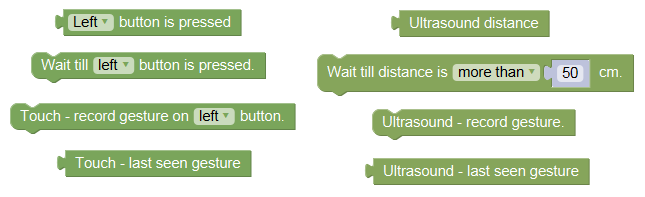
\includegraphics[]{images/sensor-blocks}}
\caption[Bloky pre ovládanie senzorov]{Bloky pre ovládanie senzorov}
\label{obr:sensor-blocks}
\end{figure}

%\begin{figure}[bh!]
%\centerline{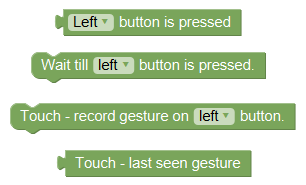
\includegraphics[]{images/touch-blocks}}
%\caption[Bloky pre ovládanie dotykových senzorov]{Bloky pre ovládanie dotykových senzorov}
%\label{obr:touch-blocks}
%\end{figure}

\newpage

\lstset{language=C,caption={Pomocná funkcia pre zaznamenanie gesta dotykovým senzorom},label=touchGestureRecordFunction,basicstyle=\footnotesize}
\begin{lstlisting}[frame=single]
void touch_gesture_record(uint8_t sensor, uint16_t time_ignore, uint16_t time_max_wait)
{
	uint16_t count = 0;
	uint8_t no_valid_gesture = 0;
	uint32_t time_start = millis();

	while ((millis() - time_start) <= time_max_wait) {
		if (digitalRead(sensor)) {
      no_valid_gesture++;
      delay(10);
      if (no_valid_gesture == 20) {
				count++;
				
        #ifdef MODULE_SOUND
				tone2(1680, 300);
        #endif

        // *** wait time_ignore OR recognise button release
        no_valid_gesture = 0;
				time_start = millis();
        while ((millis() - time_start) <= time_ignore) {
          if (!digitalRead(sensor)) {
            no_valid_gesture++;
            delay(10);
            if (no_valid_gesture == 20)
              break;
          }
					if ((millis() - time_start) >= time_max_wait) {
						TOUCH_last_seen_gesture = count;
						return;
					}
        }
				// ***
        
        no_valid_gesture = 0;
				time_start = millis();
			}
    }
	}
	TOUCH_last_seen_gesture = count;
}

\end{lstlisting}

%\begin{figure}
%\centerline{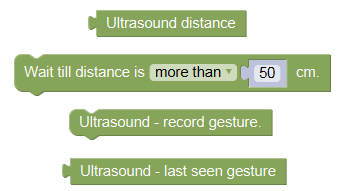
\includegraphics[]{images/ultrasound-blocks}}
%\caption[Bloky pre ovládanie ultrazvukového senzora]{Bloky pre ovládanie ultrazvukového senzora}
%\label{obr:ultrasound-blocks}
%\end{figure}


% SERIAL USB
\subsection{Sériová komunikácia prostredníctvom USB}
Bloky tejto kategórie môžete vidieť na obrázku \ref{obr:serial-blocks}. Implementované sú základné operácie pre načítanie prijatej textovej alebo číselnej hodnoty a blok pre odoslanie správy (možno ním odoslať text i číslo). Odosielanie je riešené objektom \textit{Serial}, dostupnom v jazyku Arduino. Blok pre odoslanie správy je prekladaný ako \textit{Serial.println(správa)}. Tento prístup mimo iného zabezpečí, aby všetky správy odoslané v kóde vytvorenom používateľom boli ukončené znakom konca riadku, čo nám v aplikácii umožňuje jednoznačne určiť ich hranice.

V súvislosti s prijímaním sériovej komunikácie je v Arduino implementovaný buffer. Správy sú doň uložené vždy keď prichádzajú cez sériovú linku a je na používateľovi, kedy ich prečíta. K tomuto účelu je skrze objekt \textit{Serial} k dispozícii niekoľko funkcií, ktoré ale pre mladšieho používateľa môžu pôsobiť mätúco. Implementujeme preto nad nimi abstrakciu, blok pre načítanie textu a blok pre načítanie čísla. Funkcie pre načítanie hodnoty sú blokujúce, ich volaním sa vykonávanie programu pozastaví, kým nie je prijatá textová (alebo číselná) správa. Buffer je pred volaním funkcie vždy vyprázdnený.

\begin{figure}[h!]
\centerline{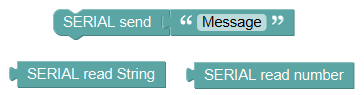
\includegraphics[]{images/serial-blocks}}
\caption[Bloky pre sériovú komunikáciu prostredníctvom USB]{Bloky pre sériovú komunikáciu prostredníctvom USB}
\label{obr:serial-blocks}
\end{figure}


%SERIAL BLUETOOTH
\subsection{Sériová komunikácia prostredníctvom Bluetooth}
Bloky tejto kategórie môžete vidieť na obrázku \ref{obr:bluetooth-blocks}. Analogicky k blokom v ponuke pre obsluhu sériovej komunikácie prostredníctvom USB tu boli definované bloky pre načítane a odoslanie číselnej alebo textovej hodnoty. Proces načítania je rovnako blokujúci, pozastaví vykonávanie programu, kým nie je prijatá správa požadovaného typu a pred týmto úkom je vždy vyprázdnený súvisiaci buffer.

\begin{figure}[bh!]
\centerline{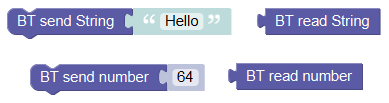
\includegraphics[]{images/bluetooth-blocks}}
\caption[Bloky pre sériovú komunikáciu prostredníctvom Bluetooth]{Bloky pre sériovú komunikáciu prostredníctvom Bluetooth}
\label{obr:bluetooth-blocks}
\end{figure}


% TIME
\subsection{Práca s časom}
Táto kategória sprístupňuje používateľovi tri bloky (obrázok \ref{obr:time-blocks}). Blok vľavo umožňuje načítať číselnú hodnotu reprezentujúcu čas v milisekundách od spustenia riadiaceho programu prístupom k Arduino funkcii \textit{millis()}. Abstrakciou nad touto funkciou vznikli bloky pre \uv{stopky}. K dispozícii sú tri nezávisle \textit{stopky}, možno ich resetovať (blok v strede na obrázku \ref{obr:time-blocks}) a načítať čas uplynutý od ich posledného resetovania (blokom vľavo na obrázku \ref{obr:time-blocks})). Implementácia je tu triviálna --- každé stopky sú premennou, \uv{reset stopiek} priradí do tejto premennej aktuálnu hodnotu \textit{millis()}, čas stopiek je vždy rozdielom aktuálnej hodnoty \textit{millis} a premennej prislúchajúcej daným \uv{stopkám}.

\begin{figure}[h!]
\centerline{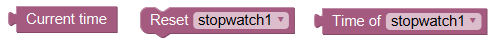
\includegraphics[]{images/time-blocks}}
\caption[Bloky pre prácu s časom]{Bloky pre prácu s časom}
\label{obr:time-blocks}
\end{figure}


% OTHER
\subsection{Kontrola batérií}
Mechanizmus umožňujúci meranie napätia batérií je súčasťou riadiaceho programu robota Otto vyvinutého pre účely denných táborov. Hodnota je cyklicky meraná a v prípade poklesu pod určitú hodnotu je robot uvedený do núdzového režimu, v ktorom ho nemožno ovládať a vybitie batérií je signalizované vydávaním melódie reprezentujúcej správu SOS. Vo verzii \textit{Otto 2020 Robotická liga} je možné takúto kontrolu ľahko integrovať do riadiaceho programu, nakoľko používateľ nemá prístup k úprave obsahu časti \textit{loop}. Implementácia tejto časti zabezpečuje, aby boli batérie kontrolované počas celého behu programu, v relatívne malých časových intervaloch.

V prípade verzie \textit{Otto 2021 Procedural} však nechávame tvorbu časti \textit{loop} čisto na používateľa. Môže v nej vytvoriť nekonečný cyklus a batérie nikdy skontrolované nebudú. Riešením je pridanie kontroly do každej, potenciálne nekonečne vykonávanej časti. Jedná sa predovšetkým o cykly \textit{while} a funkcie umožňujúce čakanie na nameranie hodnoty zo senzorov.

Používateľovi je v súvislosti s týmto mechanizmom sprístupnený blok pre načítanie hodnoty aktuálneho stavu batérií (obrázok \ref{obr:battery-block}).

\begin{figure}[h]
\centerline{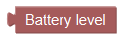
\includegraphics[]{images/battery-block}}
\caption[Bloky pre načítanie aktuálneho napätia batérií]{Bloky pre načítanie aktuálneho napätia batérií}
\label{obr:battery-block}
\end{figure}
  











